\documentclass{beamer}

\usepackage{graphicx}
\usepackage{pgfplots}

\usefonttheme{serif}

\title{1 - Binary and logic}
\author{}
\date{}

\begin{document}

\frame{\titlepage}

\begin{frame}
  \frametitle{Agenda}
  \tableofcontents
\end{frame}

\section{Inside the computer: power supply unit}

\begin{frame}
  \frametitle{Who's this? The power supply unit!}
  \begin{figure}
    \centering
    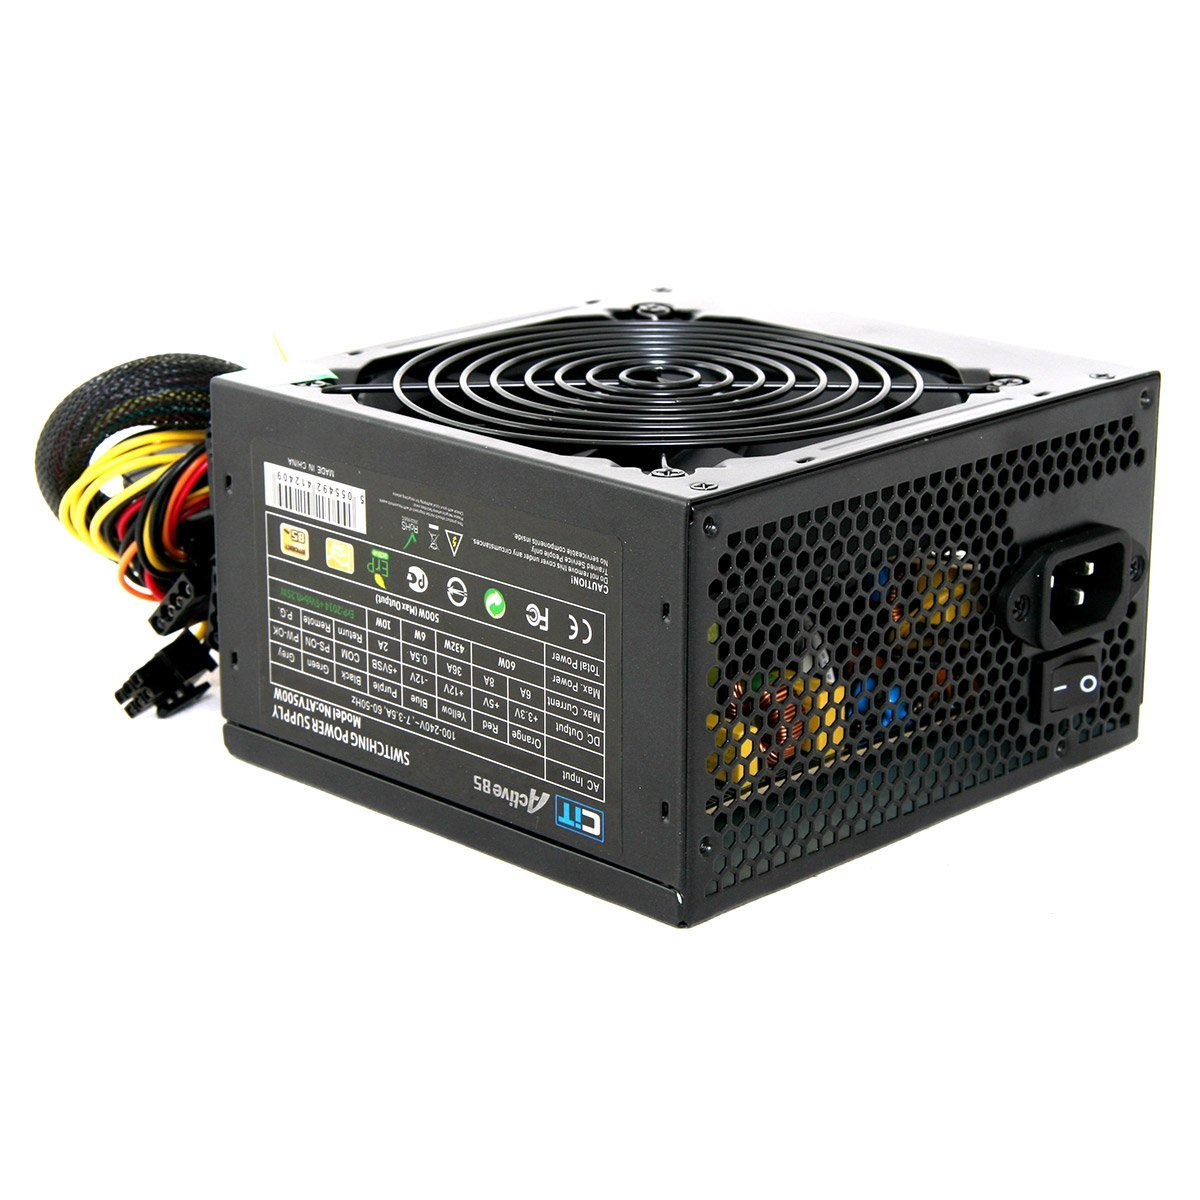
\includegraphics[width=0.4\textwidth]{res/psu.jpg} \\
    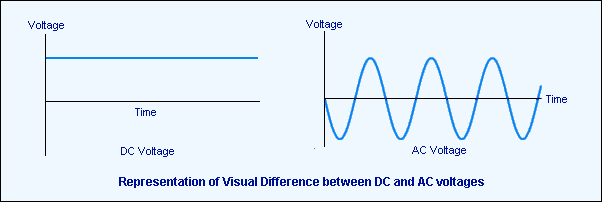
\includegraphics[width=0.8\textwidth]{res/acdc.png}
  \end{figure}

%   \begin{itemize}
%     \item
%       Converts AC in the walls, into DC for the computer.
%   \end{itemize}
\end{frame}

\section{Electricity}

\begin{frame}
  \frametitle{Electricity \& our first circuit}

  \begin{columns}
    \begin{column}{0.5\textwidth}
      \begin{center}
        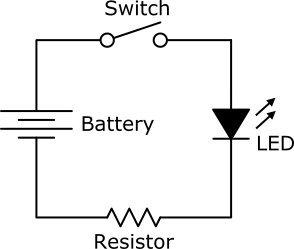
\includegraphics[width=\textwidth]{res/led-diagram.png}
      \end{center}
    \end{column}
    \begin{column}{0.5\textwidth}
      \begin{itemize}
        \item Current flows clockwise in this diagram.
        \item The battery generates direct current.
        \item We associate a positive voltage with \texttt{true} and the
          negative voltage with \texttt{false}: \emph{binary!}
        \item We can build this circuit on a \emph{breadboard.}
      \end{itemize}
    \end{column}
  \end{columns}
\end{frame}

\begin{frame}
  \frametitle{A board for cutting bread? Not really.}

  \begin{columns}
    \begin{column}{0.5\textwidth}
      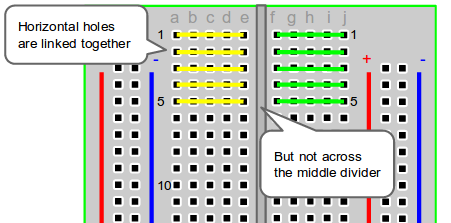
\includegraphics[width=\textwidth]{res/bb-diag.png}
    \end{column}
    \begin{column}{0.5\textwidth}
      And the holes on the left and right, called \emph{rails}, are connected vertically.
    \end{column}
  \end{columns}
\end{frame}

\section{Electronic switches: transistors}

\begin{frame}
  what's a function anyway?
\end{frame}

\section{Logic gates}

\begin{frame}
  circuits are like pzzz bang boom
\end{frame}

\end{document}
